% !TEX root = ../main.tex

\section{Learning from Data -- the Bayesian Paradigm}
\label{sec:bayes:paradigm}

At its core, the Bayesian paradigm is simple, intuitive, and compelling: for any task involving
learning from data, we start with some prior knowledge and then update that knowledge to
incorporate information from the data.  This process is known as \emph{Bayesian inference}.

Imagine we are trying to reason about some variables
or parameters $\theta$.  We can encode our initial belief as relative probabilities for different
possible instances of $\theta$, this is known as a \emph{prior} $p(\theta)$.  Given observed data
$\mathcal{D}$, we can characterize how likely different values of $\theta$ are to have given rise
to that data using a \emph{likelihood function} $p(\mathcal{D}|\theta)$.  These can then be
combined using Bayes' rule to give a \emph{posterior}, $p(\theta | \mathcal{D})$ that 
represents our updated belief about $\theta$ once the information from the data has been
incorporated
\begin{align}
	\label{eq:bayes:bayes}
	p(\theta | \mathcal{D}) = \frac{p(\mathcal{D} | \theta)p(\theta)}{\int p(\mathcal{D} | \theta)p(\theta) d\theta} 
	= \frac{p(\mathcal{D} | \theta)p(\theta)}{p(\mathcal{D})}.
\end{align}
Here the denominator, $p(\mathcal{D})$, is a normalization constant know as the \emph{marginal
	likelihood} and is necessary to ensure $p(\theta | \mathcal{D})$ is a valid probability distribution
(or probability density for continuous problems).  One can, therefore, think of Bayes' rule in the even
simpler form of the posterior being proportional to the prior times the likelihood.
For such a fundamental theorem, Bayes' rule has a remarkably simple derivation, following directly
from the product rule of probability as shown in Chapter~\ref{chp:prob}.

A key feature of Bayes' rule is that it can be used in a self-similar fashion where the posterior from
one task becomes the prior when the model is updated with more data, i.e.
\begin{align}
	\label{eq:bayes:repeat-bayes}
p(\theta | \mathcal{D}_1, \mathcal{D}_2) = 
\frac{p(\mathcal{D}_2 | \theta, \mathcal{D}_1)p(\theta | \mathcal{D}_1)}{p(\mathcal{D}_2 | \mathcal{D}_1)} =
\frac{p(\mathcal{D}_2 | \theta, \mathcal{D}_1)p(\mathcal{D}_1 | \theta) p(\theta)}
{p(\mathcal{D}_2 | \mathcal{D}_1) p(\mathcal{D}_1)} .
\end{align}
As a consequence, their is something quintessentially human about the Bayesian paradigm: we learn
from our experiences by updating our beliefs after making observations.  Our model of the world
is constantly evolving over time and is the cumulation of experiences over a lifetime.  
If we make an observation that goes against our prior experience, we do not suddenly make
drastic changes to our underlying belief, but if we see multiple corroborating observations our
view will change.
Furthermore, once we have developed
a strong prior belief about something, we can take substantial convincing to change our mind, even
if that prior belief is high illogical.  Perhaps this why humans seem to have a tendency to develop
deep-rooted prejudices.

There is similarly something distinctively Bayesian to the scientific process itself.  In science, we construct models
to explain observed phenomena and then run experiments to validate how well our model matches
real observations.  We then update and improve our model accordingly in a never-ending process of
increasing understanding for the world around us.  We can never hope to truly understand the workings
of the universe  -- after all, it is, at least for practical purposes, fundamentally random~\citep{rainforth2013random} 
-- and so we can hope only to construct increasingly accurate and pertinent models.
This sequential updating, at the very least, shares parallels with the process of Bayesian modeling
and could be argued to be a fundamentally Bayesian process in its own right.

To give a more concrete example of Bayesian modeling consider estimating
the probability of getting a heads from a weighted coin.  Let's call this weighting $\theta \in [0,1]$ such
that the probability of getting a heads  ($H$)  when flipping the coin is $p(Y=H | \theta)=\theta$
where $Y$ is the outcome of the flip.  This will be our likelihood function, corresponding to a
\emph{Bernoulli} distribution, noting that the probability
of getting a tails ($T$) is $p(Y = T | \theta) = 1-\theta$.
Before seeing the coin being flipped we have some prior belief about its weighting.  We
can, therefore, define a prior $p(\theta)$, for which we take the beta distribution
\begin{align}
\label{eq:bayes:beta}
p(\theta) = \textsc{Beta}\left(\theta ; \alpha,\beta\right) = \frac{\Gamma(\alpha+\beta)}{\Gamma (\alpha) \Gamma(\beta)}
\theta^{\alpha-1} (1-\theta)^{\beta-1}
\end{align}
where $\Gamma(\cdot)$ is the gamma function and we will take $\alpha=\beta=2$.  
A plot for this prior is shown in Figure~\ref{fig:inf:coin_flip:0}
where we see that under our prior then it is more probable that $\theta$ is close to $0.5$ than the
extremes $0$ and $1$.  

Now imagine that we flip the coin and get a tails ($T$).  We can
use our prior and likelihood to calculate the posterior
\begin{align}
p(\theta | Y_1 = T) &= \frac{p(\theta) p(Y_1=T | \theta)}{\int p(\theta) p(Y_1=T | \theta) d\theta} = \frac{\theta (1-\theta)^2}{\int \theta (1-\theta)^2 d\theta} \nonumber \\
&= \textsc{Beta}\left(\theta ; 2,3\right) = 
\frac{\Gamma(\alpha+\beta)}{\Gamma (\alpha) \Gamma(\beta)} \theta (1-\theta)^2 \label{eq:prob:beta_post_1}.
\end{align}
Here we have used the fact that a Beta prior is \emph{conjugate} to a Bernoulli likelihood
to give an analytic solution.  Conjugacy means that the prior-likelihood combination gives
a posterior that is of the same form as the prior distribution.  More generally, for a prior of
$\textsc{Beta}(\theta ; \alpha, \beta)$ then the posterior will be $\textsc{Beta}(\theta ; \alpha+1, \beta)$
if we observe a heads and $\textsc{Beta}(\theta ; \alpha, \beta+1)$ if we observe a tails.
Figure~\ref{fig:inf:coin_flip:1} shows that our
posterior incorporates the information from the prior and the observed data.  Namely, our observations 
mean the distribution
has drifted towards it being more probable that $\theta<0.5$.  The posterior
also reflects the fact that we are still uncertain about the value of $\theta$, it is not simply the
empirical average of our observations which would give $\theta=0$.

\begin{figure}[t]
	\centering
	\begin{subfigure}[t]{0.24\textwidth}
		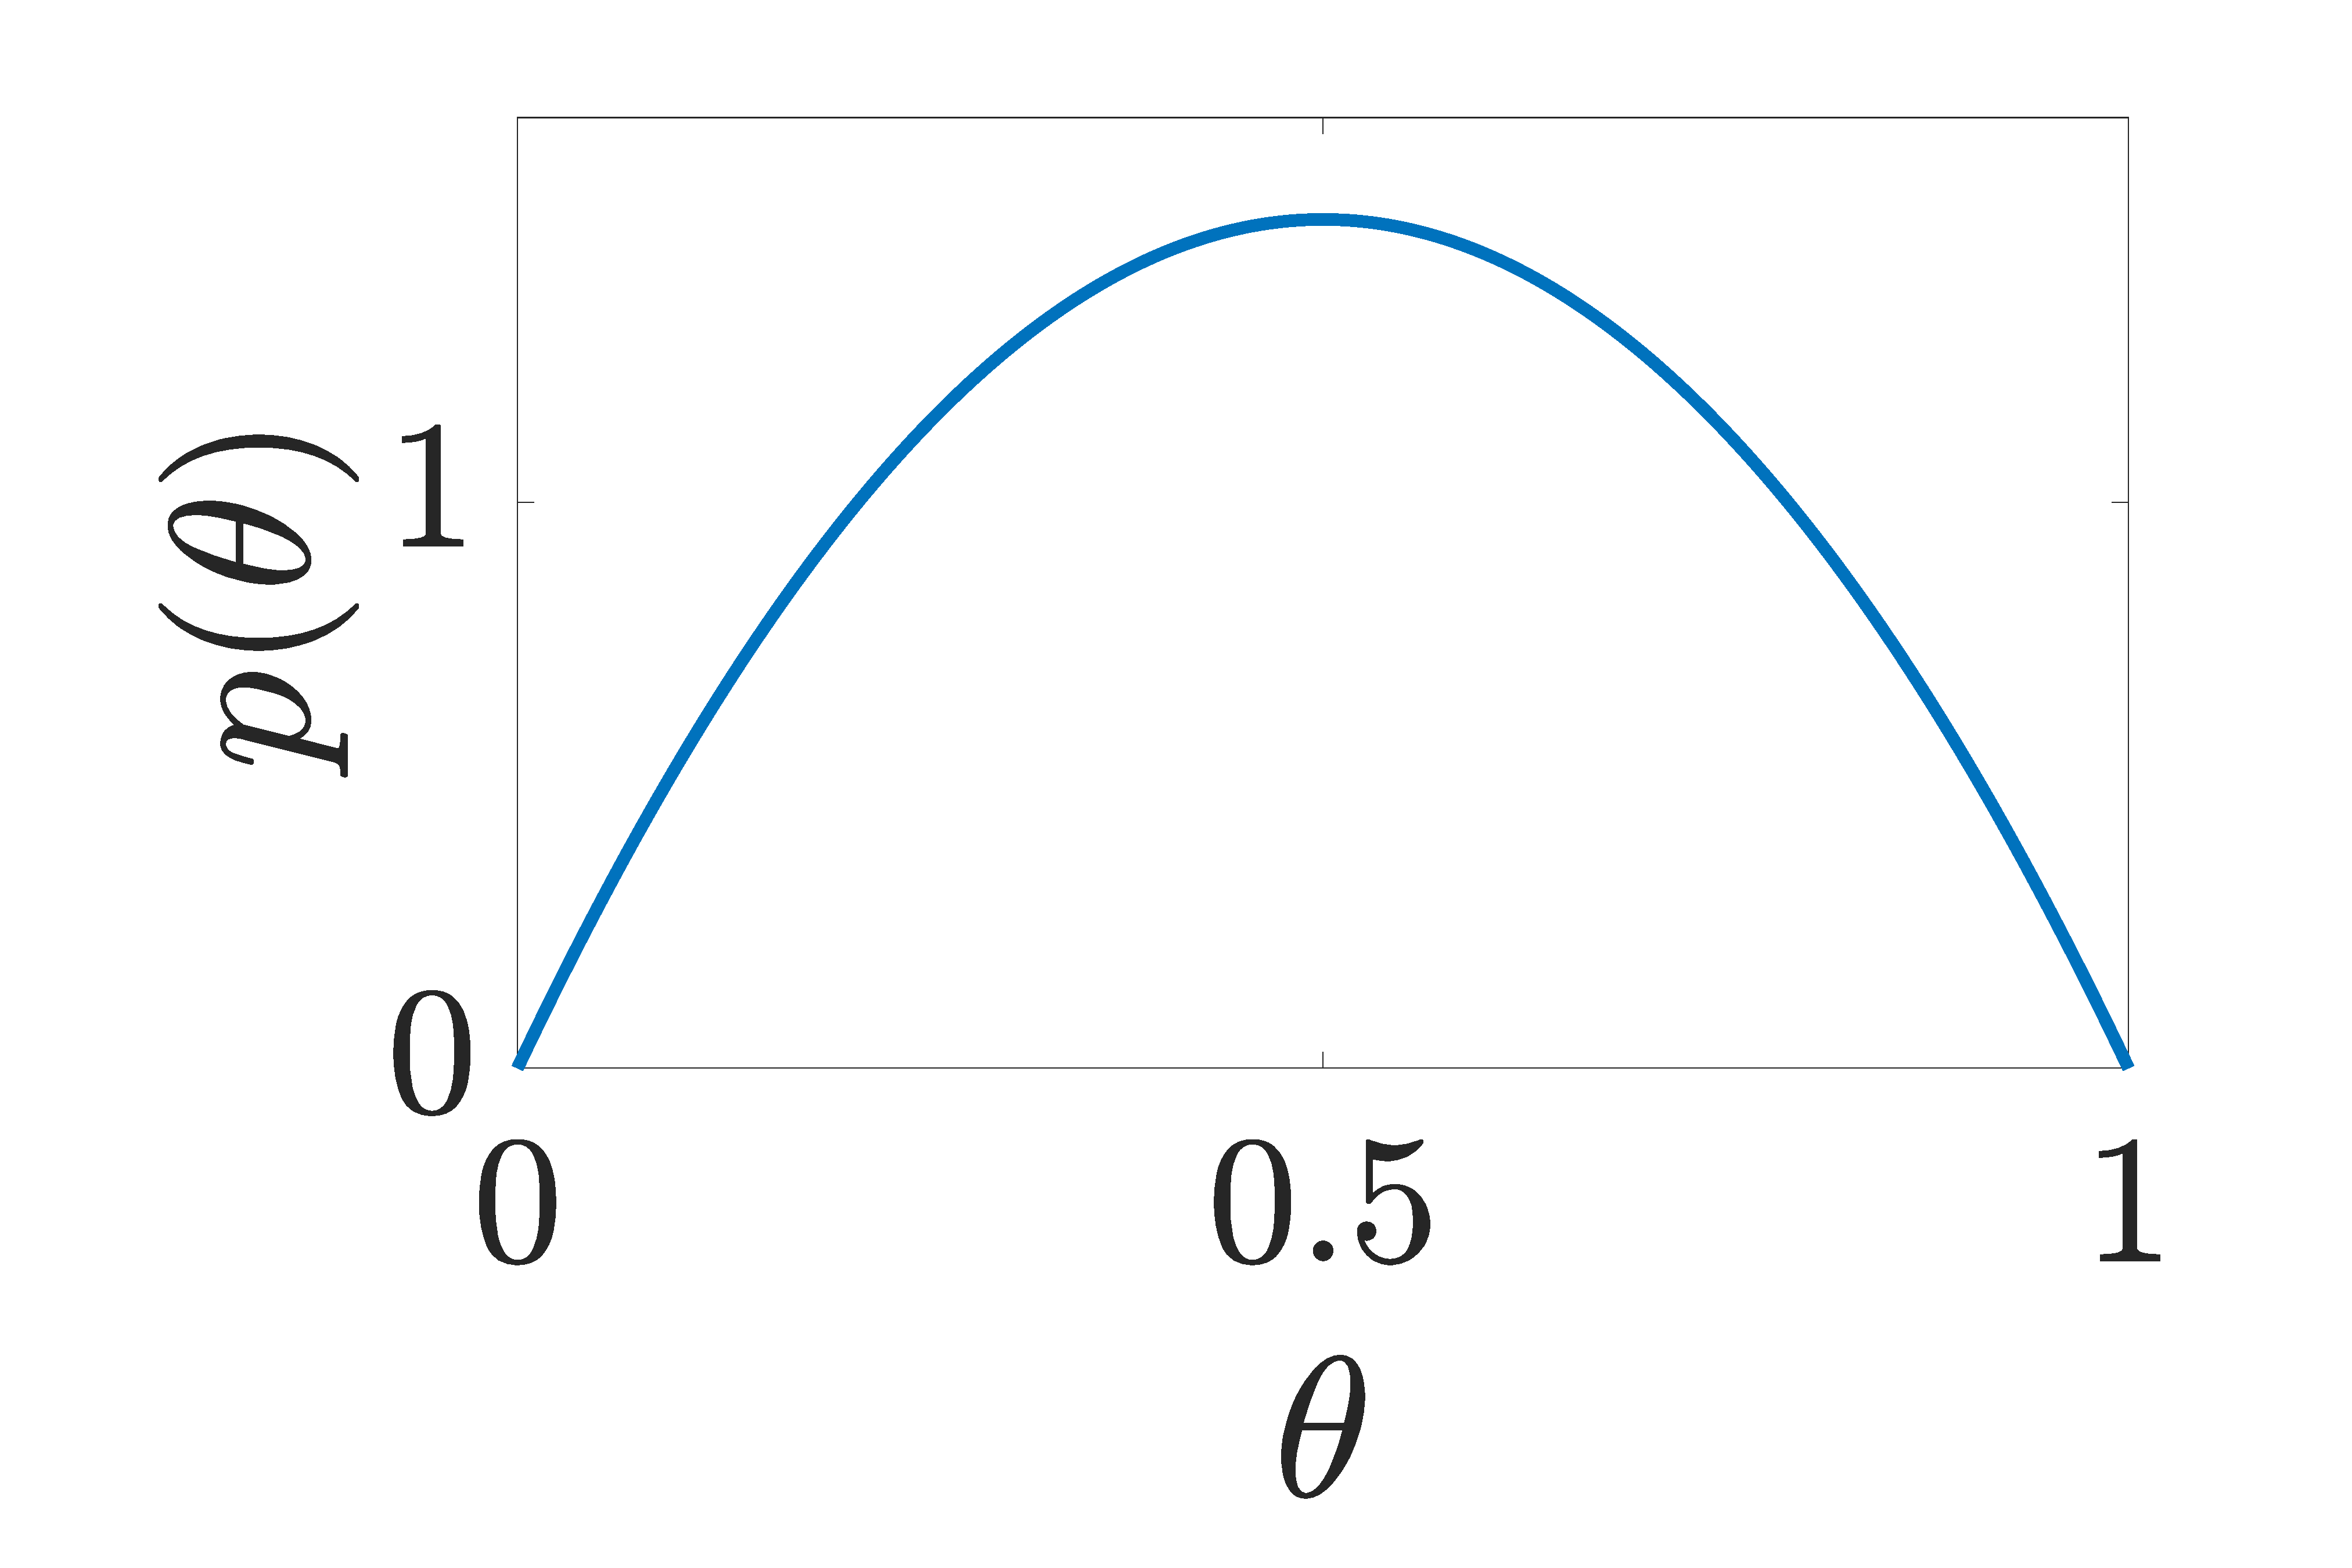
\includegraphics[width=\textwidth]{coin_flip_0}
		\caption{Prior \label{fig:inf:coin_flip:0}}
	\end{subfigure}
	\begin{subfigure}[t]{0.24\textwidth}
		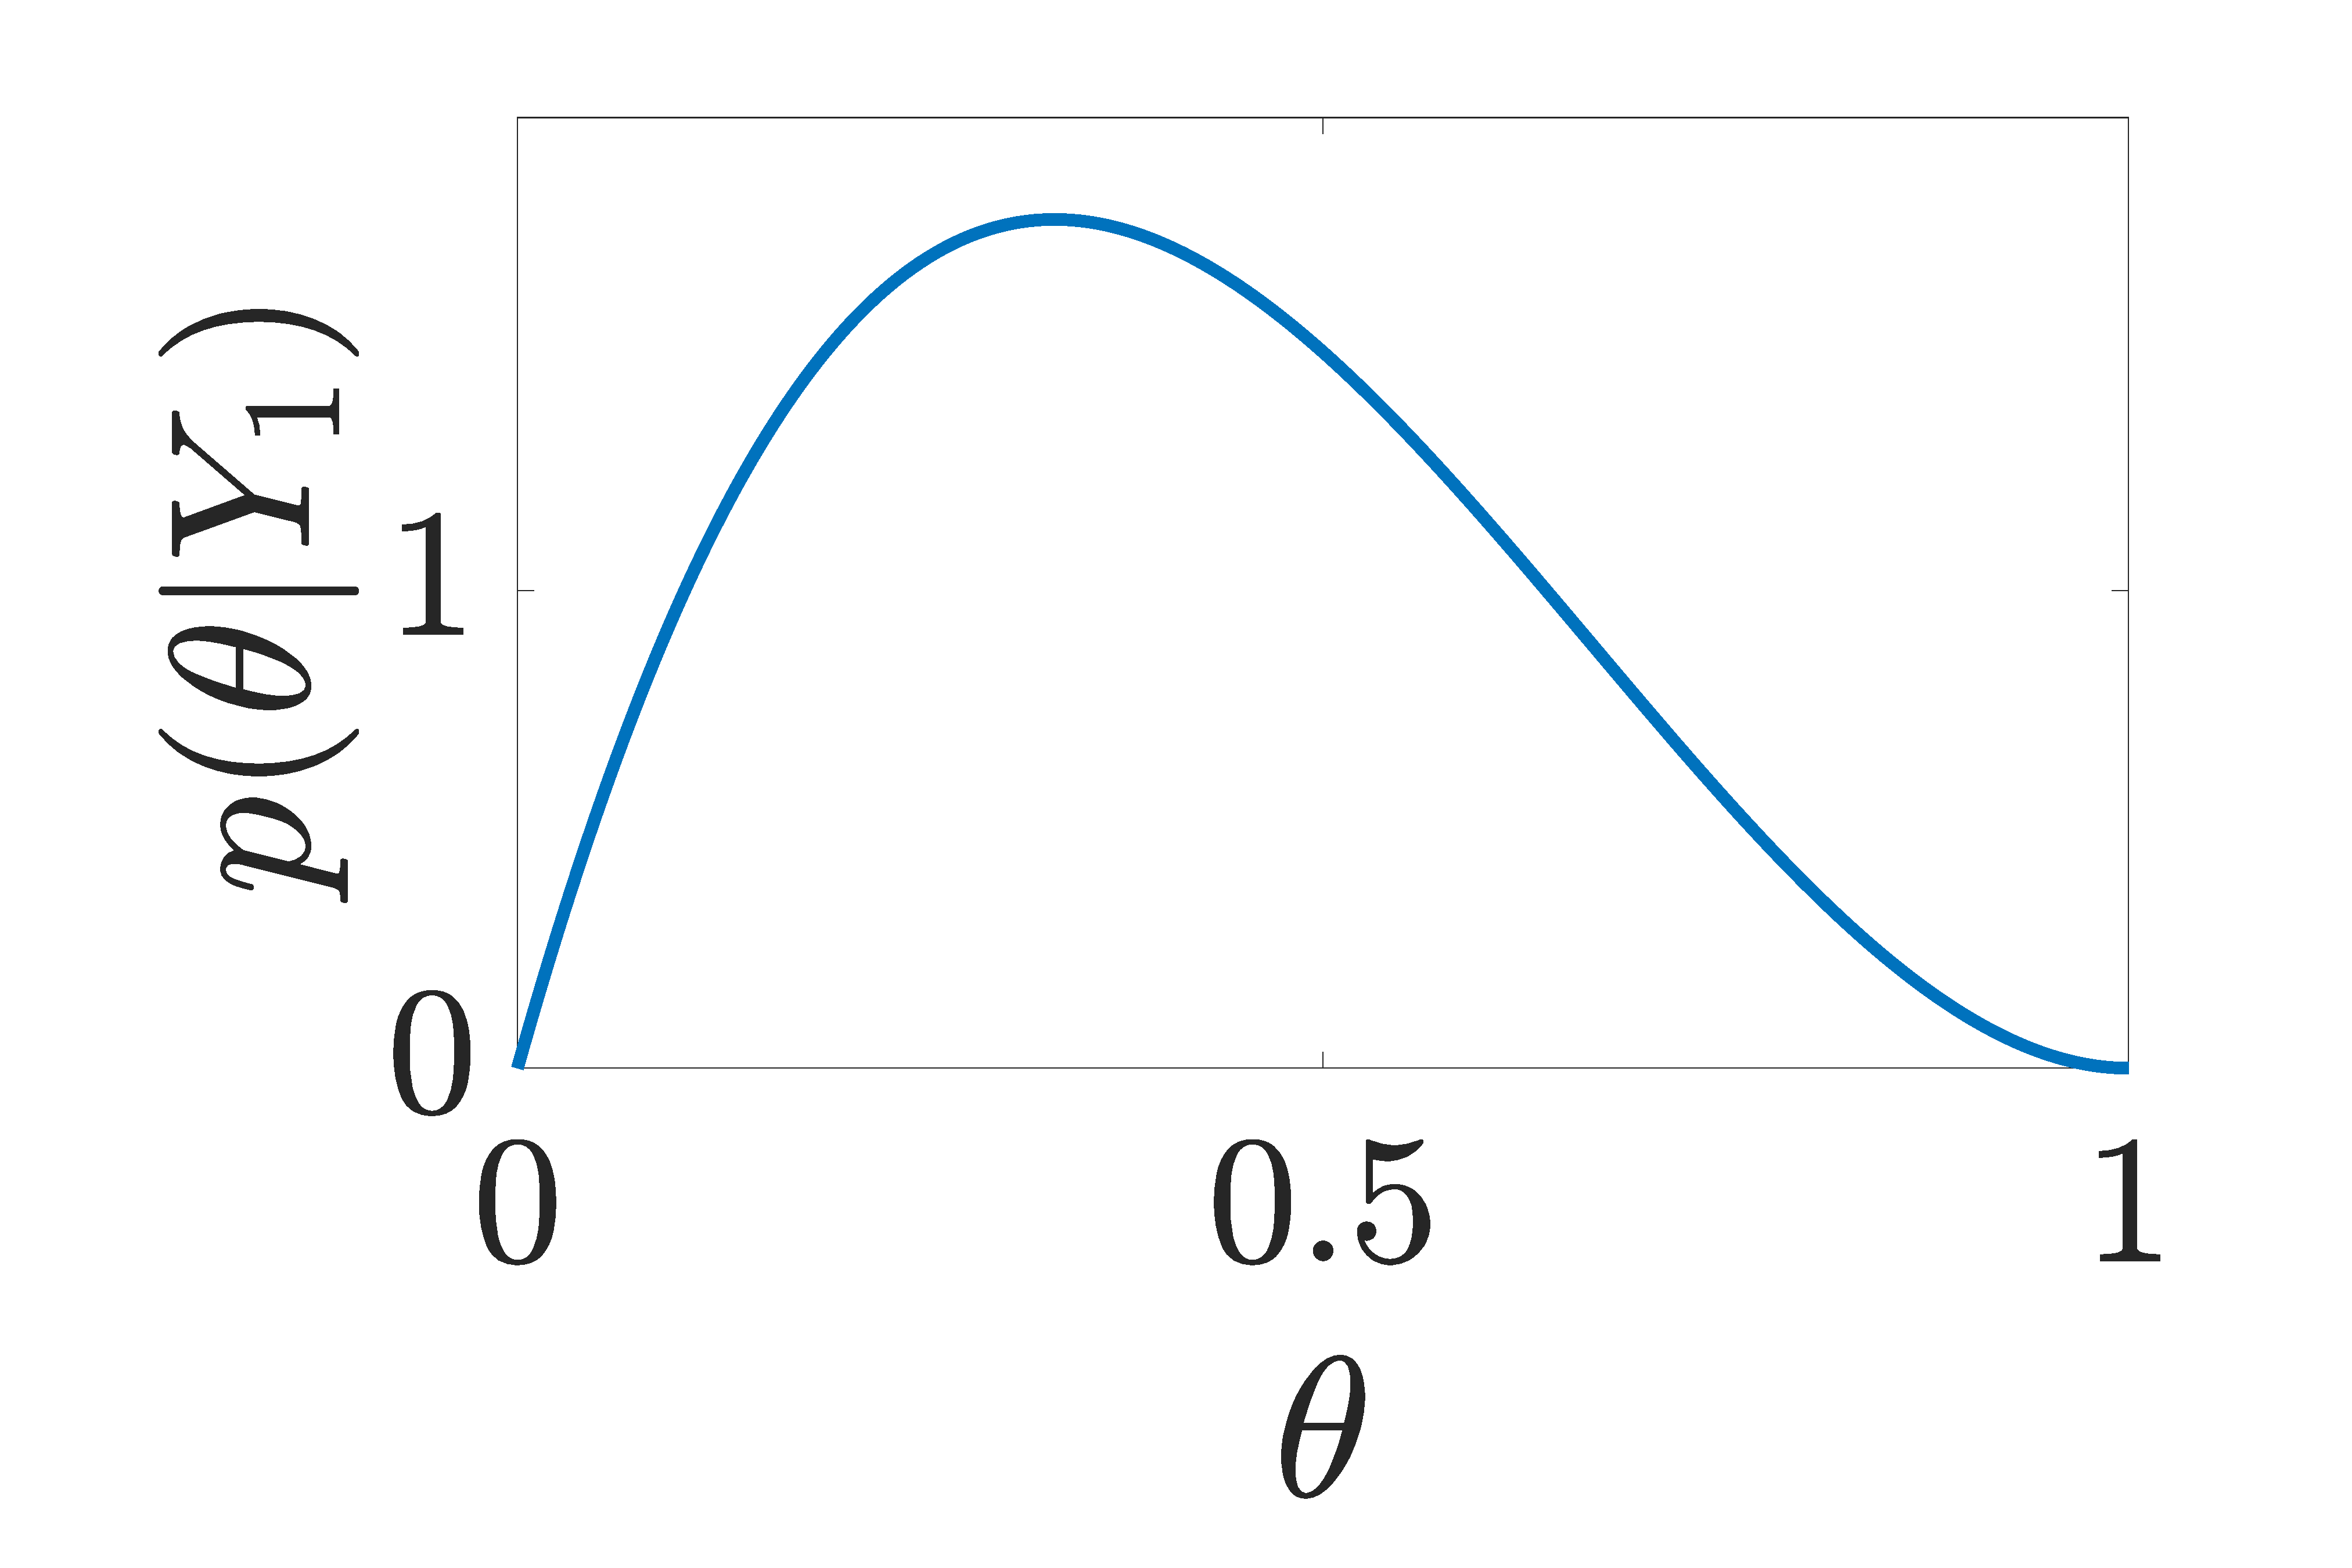
\includegraphics[width=\textwidth]{coin_flip_1}
		\caption{Posterior 1 flip \label{fig:inf:coin_flip:1}}
	\end{subfigure}
	\begin{subfigure}[t]{0.24\textwidth}
		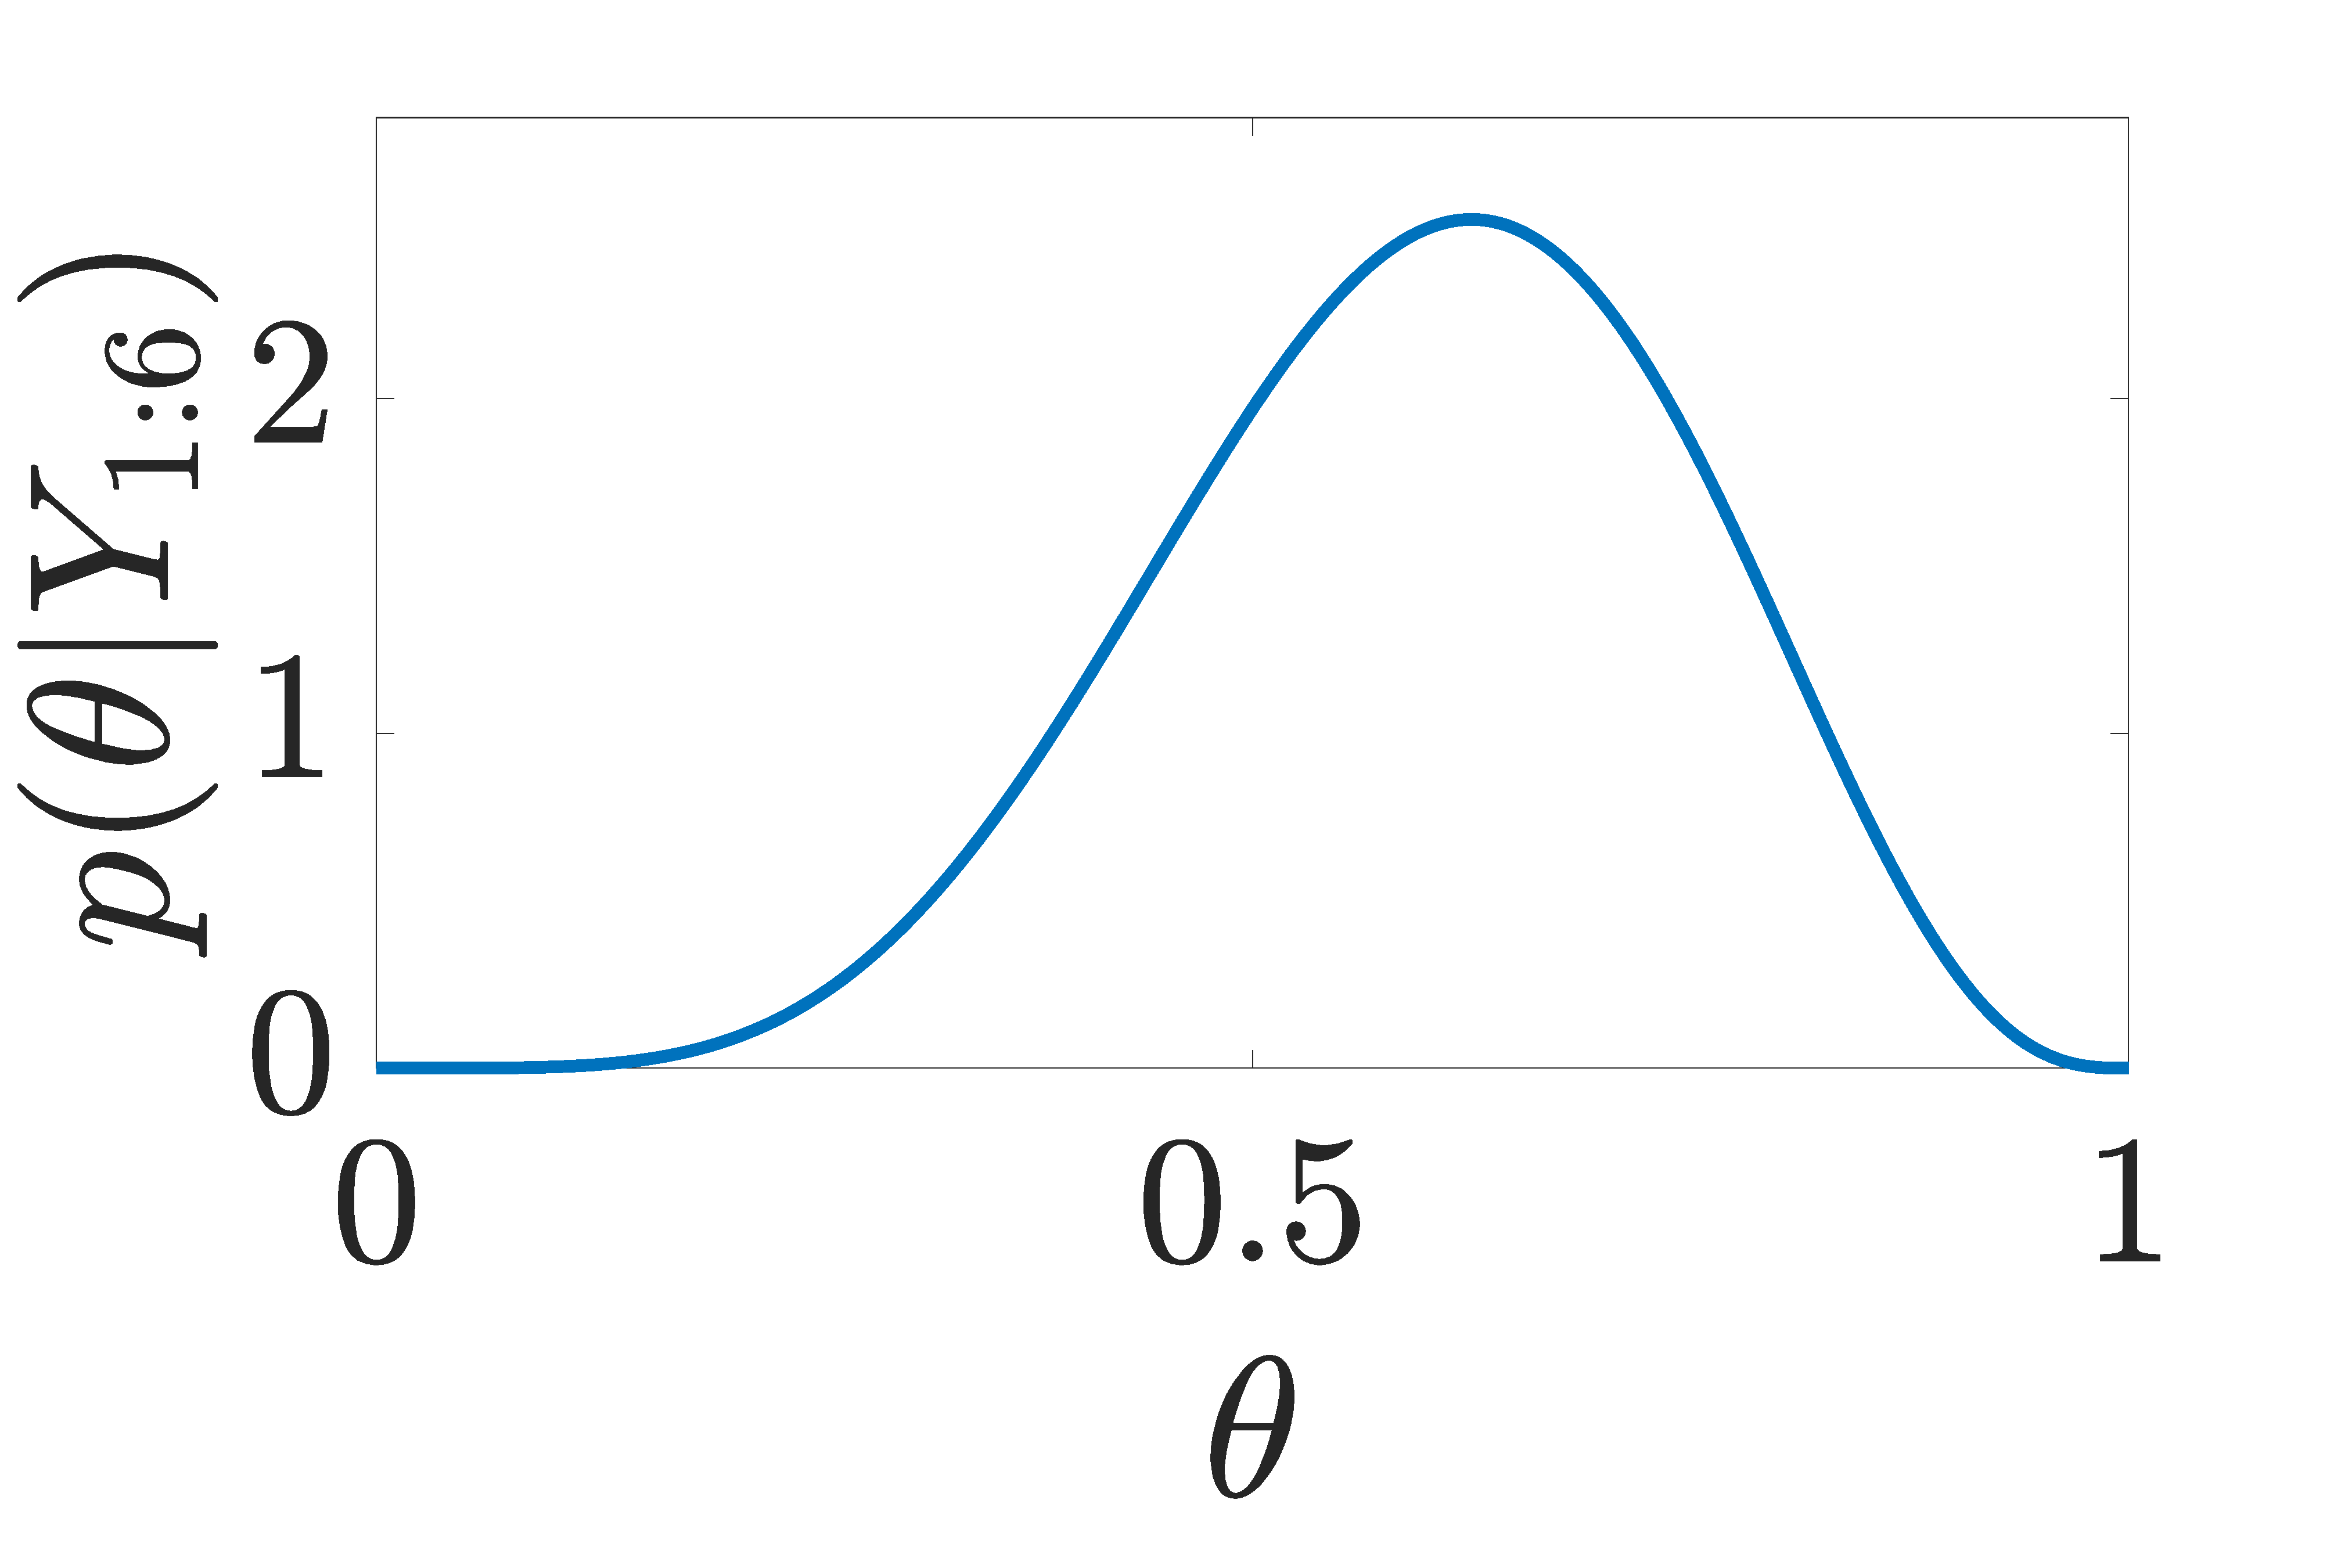
\includegraphics[width=\textwidth]{coin_flip_6}
		\caption{Posterior 6 flips \label{fig:inf:coin_flip:6}}
	\end{subfigure}
	\begin{subfigure}[t]{0.24\textwidth}
		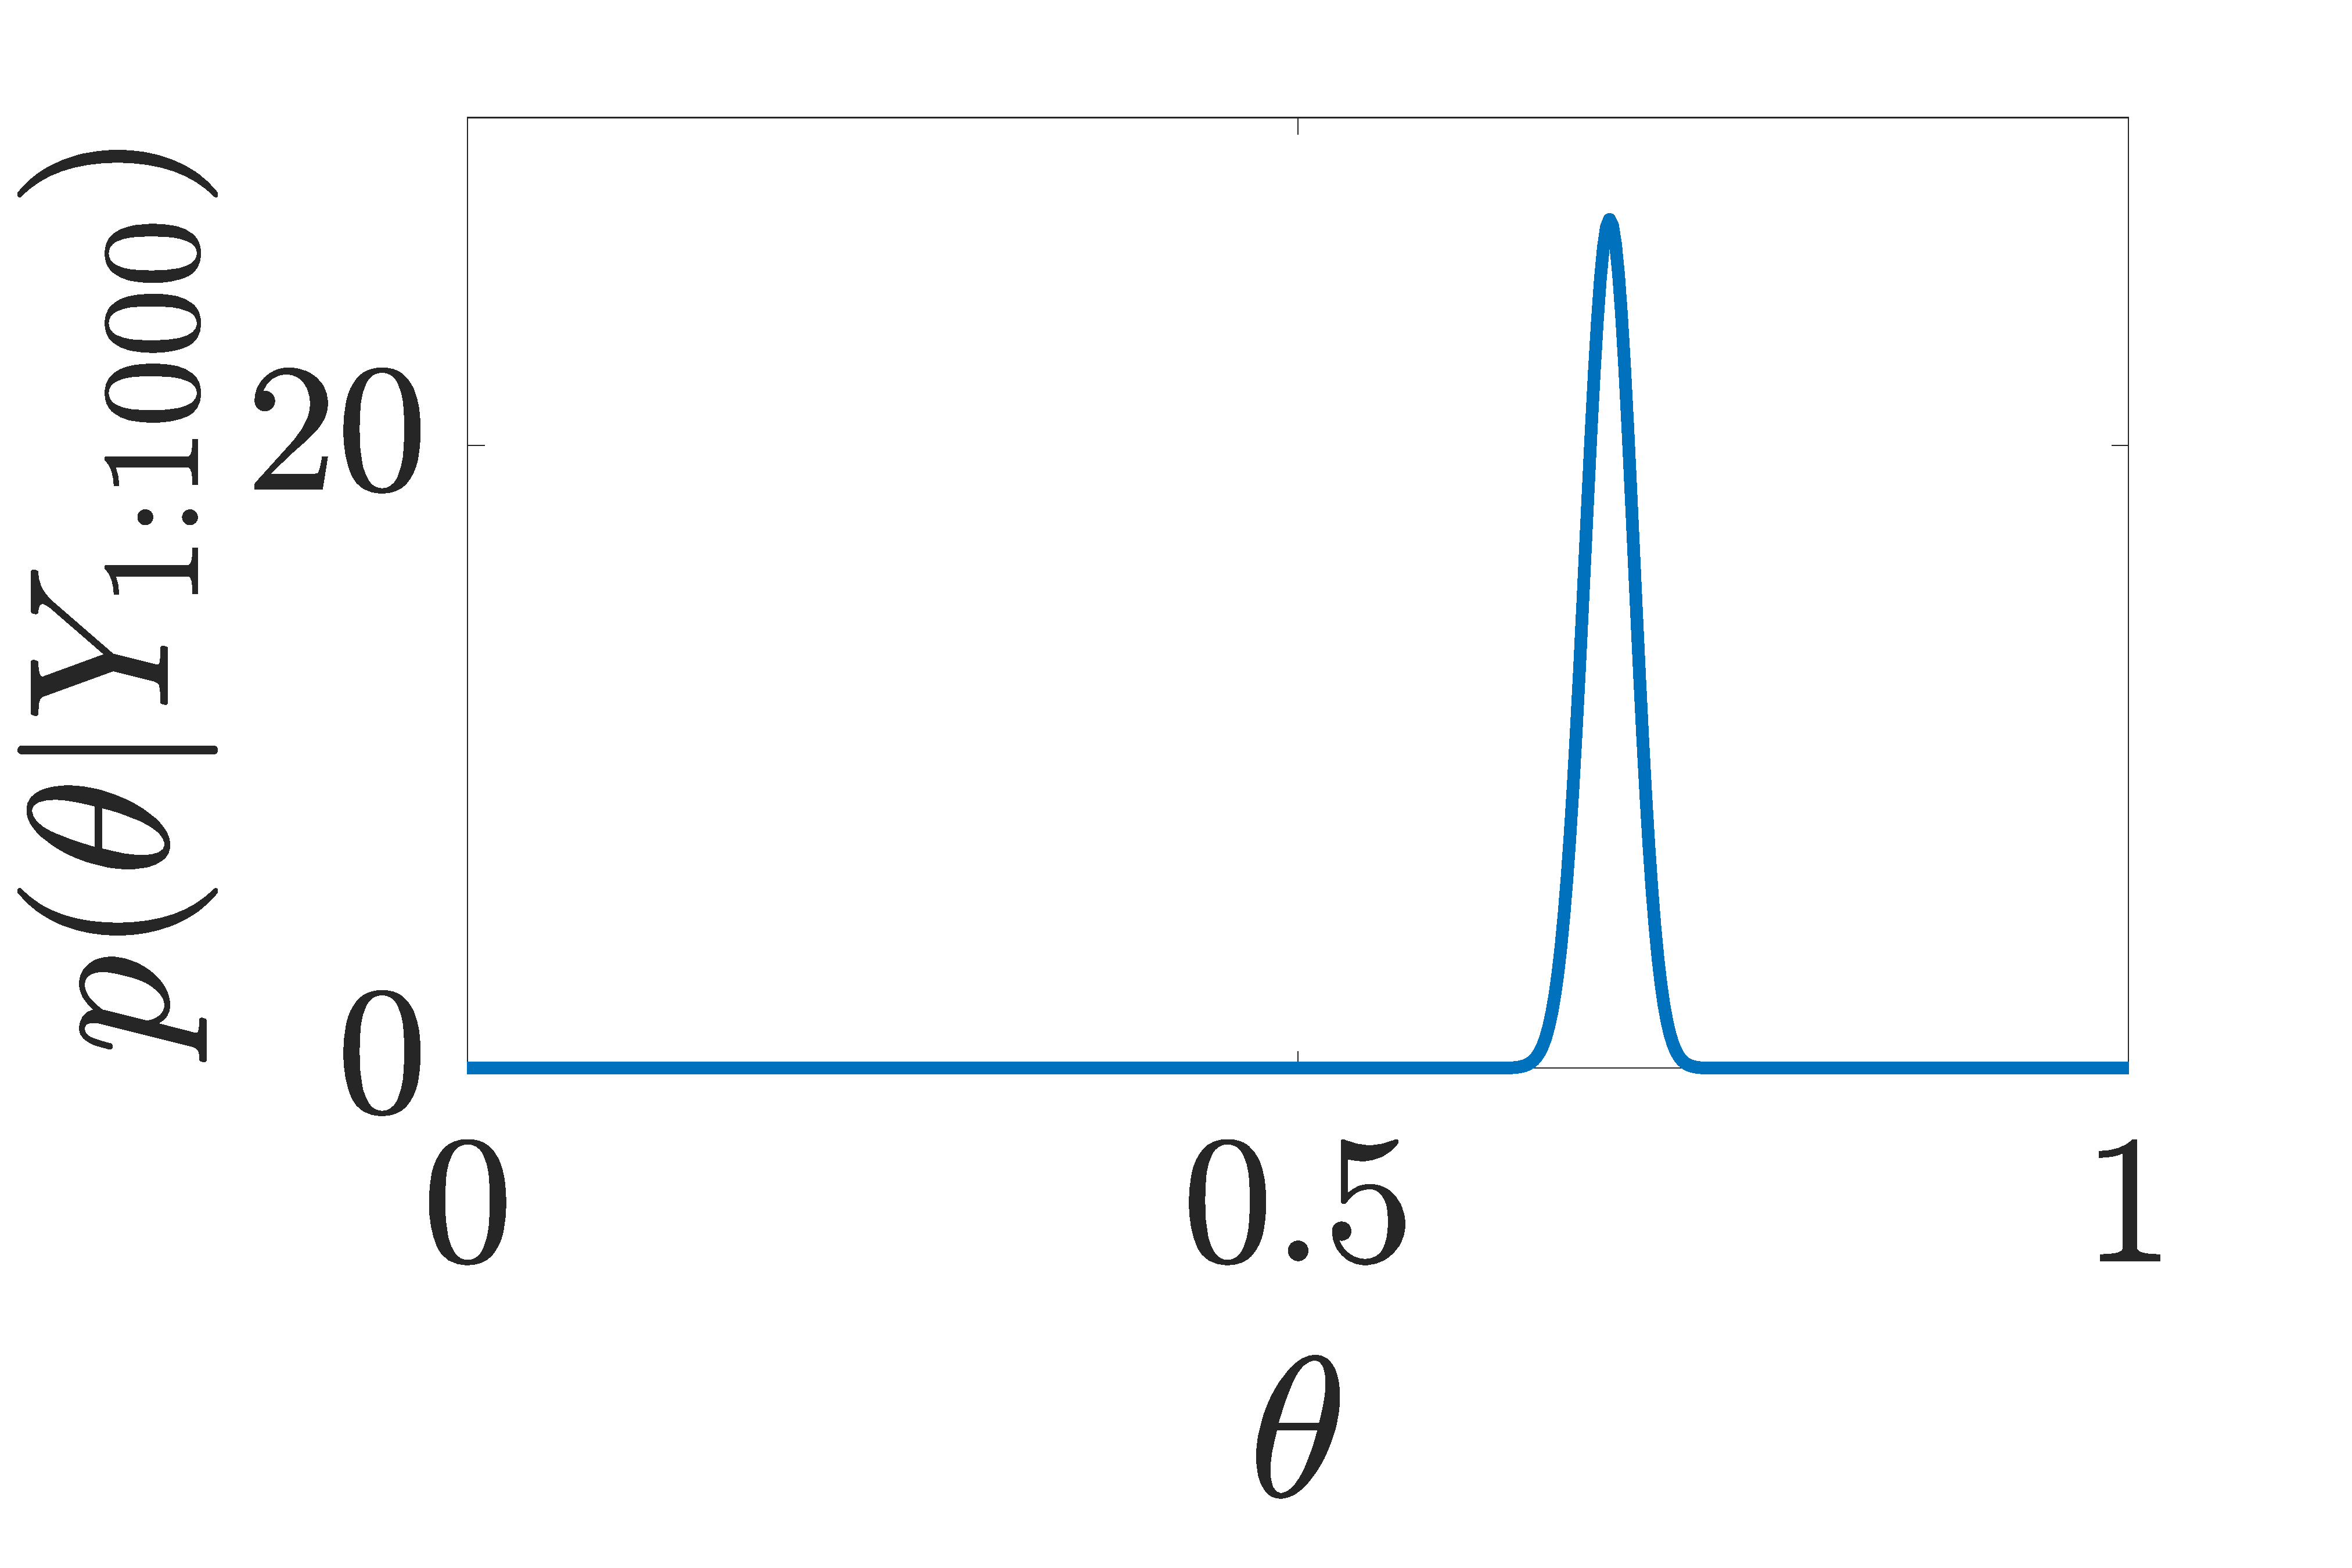
\includegraphics[width=\textwidth]{coin_flip_1000}
		\caption{Posterior 1000 flips \label{fig:inf:coin_flip:1000}}
	\end{subfigure}
	\caption{Prior and posteriors for coin flip example after different numbers
		of observations.
		\label{fig:inf:coin_flip}}
\end{figure}

If we now flip the coin again, our previous posterior~\eqref{eq:prob:beta_post_1} becomes our
prior and we can incorporate the new observations in the same way.  
Through our previous conjugacy result, then if we observe $n_{H}$ heads
and $n_{T}$ tails and our prior is $\textsc{Beta}(\theta ; \alpha, \beta)$ then our posterior is
$\textsc{Beta}(\theta ; \alpha+n_H, \beta+n_T)$.
Thus if our sequence of new
observations is $HTHHH$ then our new posterior is
\begin{align}
p(\theta | Y_1,\dots,Y_6) = \frac{p(Y_2,\dots,Y_6 | \theta)p(\theta | Y_1)}
{\int p(Y_2,\dots,Y_6 | \theta)p(\theta | Y_1) d\theta} = \textsc{Beta}\left(\theta ; 6,4\right),
\end{align}
which is shown in Figure~\ref{fig:inf:coin_flip:6}.  We see now that our belief for the probability of heads
has shifted higher and that the uncertain has reduced because of the increased number
of observations.
After seeing a total of $1000$ observations as shown in Figure~\ref{fig:inf:coin_flip:1000}, we
see that the posterior has predominantly collapsed down to a small range of $\theta$,
close to the true value of $\theta$ which happens to be $0.7$.

Now we have combined  our prior information with the information from data, a natural
next question is how can we use this to make predictions.  In the Bayesian setting,
this is done with the posterior predictive distribution which marginalizes out over
the parameters.  For the coin flip case we have
\begin{align}
\label{eq:bayes:post-pred}
p( Y_{N+1}=H | Y_{1:N}) &= \int p(Y_{N+1}=H, \theta | Y_{1:N}) d\theta
= \int p(Y_{N+1}=H | \theta) p(\theta | Y_{1:N})  d\theta \nonumber \\
&= \int  \theta \; \textsc{Beta}(\theta ; \alpha+n_H, \beta+n_T) d\theta 
%= \int  
%\frac{\Gamma(\alpha+\beta)}{\Gamma (\alpha) \Gamma(\beta)} 
%\theta^{\alpha} (1-\theta)^{\beta-1} d\theta = 
%\frac{\Gamma(\alpha+\beta) \Gamma (\alpha+1)}{\Gamma (\alpha) \Gamma(\alpha+1+\beta)} \nonumber \\
=\frac{\alpha+n_H}{\alpha+n_H+\beta+n_T}
\end{align}
where we have used the known result for the mean of the Beta distribution.
The role of the parameters $\alpha$ and $\beta$ in our prior now become apparent
-- they take on the role of pseudo-observations.  Our prediction is in line with the
empirical average from seeing $\alpha+n_H$ heads and $\beta+n_T$ tails.  The larger
$\alpha+\beta$ is then the strong our prior compared to the observations, while we
can skew towards heads or tails being more likely by changing the relative values of $\alpha$
and $\beta$.

More generally the posterior predictive distribution will depend on a queried input point.
To demonstrate this, consider the example of a Bayesian linear regression from inputs $x\in\real^D$
to outputs $y\in\real^D$.  Assume that we have seen $N$ observations $\mathcal{D} = \{x_n,y_n\}_{n=1}^N$
and let $\mathbf{x}=[x_1,\dots,x_N]^T$ and $\mathbf{y}=[y_1,\dots,y_N]^T$ respectively be 
a $N\times D$ matrix and a column vector whose rows correspond to the different data points.
Our regression is of the form $y_n= x_n^T\mathbf{w}+b+\epsilon_n$ where $\mathbf{w}\in\real^D$, $b\in\real$
and each $\epsilon_n \iid \mathcal{N}(0,\sigma^2)$.  This implies a likelihood of
\begin{align}
\label{eq:bayes:linear-reg-lik}
p(\mathbf{y}|\mathbf{x},\mathbf{w},b,\sigma) = \prod_{n=1}^{N} p(y_n | x_n, \mathbf{w}, b, \sigma) = 
\prod_{n=1}^{N} \mathcal{N}(y_n;x_n^T\mathbf{w}+b,\sigma^2).
\end{align}
For simplicity we will assume that $\sigma$ and $b$ are known fixed parameters,
but we will put a prior on $\mathbf{w}$ as follows in order to perform inference
%\begin{subequations}
%\label{eq:bayes:linear-reg-prior}
\begin{align}
\label{eq:bayes:linear-reg-w}
p(\mathbf{w}) &= \mathcal{N}(\mathbf{w};\mathbf{0},C)
%\\
%\label{eq:bayes:linear-reg-b}
%p(b) &= \mathcal{N}(b;0,s^2),
\end{align}
%\end{subequations}
where $C$ is a fixed covariance matrix.
%% and $s$ a fixed scalar standard deviation.
%We further assume that $p(\mathbf{w},b | \sigma) = p(\mathbf{w}) p(b) $, i.e. that all
%three parameters are independent under the prior.
To make predictions, we first calculate the posterior
\begin{align}
p(\mathbf{w}| \mathcal{D}, b,\sigma) &= \mathcal{N}(\mathbf{w};\mathbf{0},C)
\prod_{n=1}^{N} \mathcal{N}(y_n;x_n^T \mathbf{w}+b,\sigma^2) \nonumber \\
&= \mathcal{N}\left(\mathbf{w} ; m, S\right) \\
\mathrm{where} \quad m &= S^{-1} \mathbf{x}^T \left(\mathbf{y}-b\right)/\sigma^2, \nonumber \\
S &= \left( C^{-1}+\frac{\mathbf{x}^T\mathbf{x}}{\sigma^2}\right)^{-1}. \nonumber
%&= \mathcal{N}\left(\mathbf{w} ; \left( C^{-1}+\frac{\mathbf{x}^T\mathbf{x}}{\sigma^2}\right)^{-1} 
%\frac{\mathbf{x}^T \left(\mathbf{y}-b\right)}{\sigma^2},
%\left( C^{-1}+\frac{\mathbf{x}^T\mathbf{x}}{\sigma^2}\right)^{-1} \right),
\end{align}
We have omitted the necessary linear algebra (see for example~\cite{bishop2006pattern}
Sections 2.3.3 and 3.3)
but note the conjugacy between
the normal distribution and itself.  Prediction now uses the posterior predictive, marginalizing
over the parameters in the same manner as the coin flip example.  Here though, we are interested
in predicting the output $\tilde{y}$ at a particular input point $\tilde{x}$ for which we have
\begin{align}
p(\tilde{y}| \tilde{x},\mathcal{D}, b,\sigma) &= \int p(\tilde{y}| \tilde{x},\mathbf{w}) 
p(\mathbf{w}| \mathcal{D}, b,\sigma) d\mathbf{w} 
= \int \mathcal{N}(\tilde{y};\tilde{x}^T\mathbf{w}+b,\sigma^2)
\mathcal{N}\left(\mathbf{w} ; m, S\right) d\mathbf{w} \nonumber \\
&= \mathcal{N} \left(\tilde{y} \; ; \;\tilde{x}^Tm+b, \; \tilde{x}^T S^{-1}\tilde{x}+\frac{1}{\sigma^2} \right)
\end{align}
which again follows from standard results for Gaussian distributions.  We therefore have
an analytic predictive distribution at any possible input point.
Though this linear regression example might seem overly simple for practical purposes, we
will see in Section~\ref{sec:opt:GPs} that substantially more advanced models, such as
Gaussian processes, can be viewed as linear regressions between a set of features on the inputs $\phi(x)$
and the output $y$.

The models we have introduced so far are specific examples of Bayesian modeling and will
clearly only be applicable or appropriate in very particular scenarios.  However, the only restrictions we
have in order to carry out Bayesian modeling is that the prior and likelihood are valid probability distributions
(in practice even these requirements can often be relaxed).  Bayesian modeling is at its heart a
generative approach and its real power will be when we design a rich and expressive \emph{generative model} 
that reflects our application specific knowledge.  In other words, we can define our model
by carefully constructing a stochastic process that describes how the data and parameters are generated.
This model then corresponds to the joint distribution $p(\theta,\mathcal{D})$.
We can then think of providing real data as refining our model, providing an updated distribution
on the parameters and subsequent predictions that incorporate the information from the data.  The more
flexible we make our generative model, the more we can make it represent the our data.  The less flexible
we make the generative model, the more weighting is given to our prior assumptions.

To give an intuitive example of such a generative approach, consider the problem of identifying objects in
a visual scene.  Here it is relatively straightforward to construct a model for generating images by
constructing a sampler for which objects appear in the scene and their respective positions.  Such
graphics generators are used for computer games all the time.  Here our parameters are the objects and
the data is the image.  Bayesian inference can now be thought of as the process of \emph{inverting} our generator:
given objects we can generate images but we want to identify objects from images.  We will return
to these ideas in Chapter~\ref{chp:probprog} where we show how, using probabilistic programming,
one can think of all stochastic simulators as defining Bayesian models and as the process of inference as
inverting these simulators.